%! Author = Saeid Yazdani
%! Date = 7/26/2024


\section{Ganged-Mode Operation}
\label{sec:ganged-mode-operation}

The \ac{ATE} under investigation contains multiple \ac{DPS} units, each rated
at \SI{500}{\milli\ampere} maximum \acs{DC} current.
To supply larger currents to a \ac{DUT} with higher current demand,
multiple \ac{DPS} units must be connected in parallel
(so-called ganged mode) to increase the current output of the \ac{ATE}.

Ganged mode in power supplies is a configuration where multiple power supply
units are connected and operated together to form a cohesive system.
This mode of operation is designed to increase the total available
current in the form of load-sharing.
However, implementing gang mode comes with major challenges:

\begin{itemize}[topsep=8pt,itemsep=4pt,partopsep=4pt, parsep=4pt]
    \item \textbf{Complexity:}
    Design and implementation of a ganged configuration are more complex
    and requires much more wiring and components compared to a single power
    supply with higher output power.
    Precise calibration and voltage regulation also increases the design
    complexity.
    In addition, the overall software and firmware of the \ac{ATE} must
    be more sophisticated and therefore more error-prone.

    \item \textbf{Synchronization:}
    A perfect load balancing between multiple \ac{DPS} units in parallel is hard
    to achieve and can result in under-utilization or over-utilization of units.

    \item \textbf{Stability:}
    Small differences in output voltage between power supplies can result in
    circulating currents, leading to oscillations and instability
    due to subtle differences in impedance and phase angles caused by
    manufacturing tolerances which can not guarantee each participating
    \ac{DPS} in a ganged configuration to be exactly the same as others.
    Differences in transient response can also be expected if the participating
    units are not electrically matching.

    \item \textbf{\acs{EMI} Susceptibility:}
    Additional wiring and multiple power supplies can introduce noise and
    electromagnetic interference, which may affect the accuracy and
    performance of the ATE system and potentially couple into the \ac{DUT}.

    \item \textbf{Thermal management:}
    Multiple power supplies generate more heat, necessitating a robust
    cooling solution for the \ac{ATE}.
    Inadequate thermal management can lead to overheating and hinders the
    reliability and performance of the \ac{ATE}.

    \item \textbf{Cost:}
    More component count means higher production cost and higher maintenance
    cost are to be expected as identifying and troubleshooting issues can be
    more complex and time-consuming compared to a single power supply system.

\end{itemize}

\autoref{fig:ganged-mode-dps-structure} shows the block diagram of the DPS gang
configuration in the target \ac{ATE}.
In this mode, a DPS uses a master channel and one or more slave channels in
parallel to increase current output.
The master channel controls the output stages of the slave channels by
switching out their control amplifiers and connecting its own control amplifier
to them.

\begin{figure}[h]
    \centering
    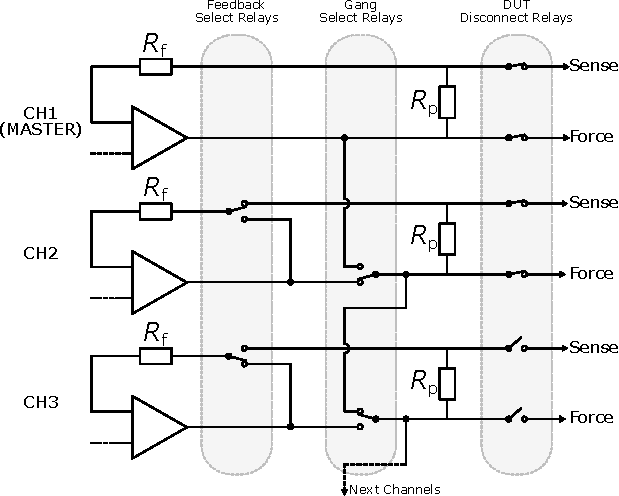
\includegraphics[width=0.9\textwidth]
    {figures/diagonostics/ganged_dps}
    \caption[Ganged DPS Structure]{
        Simplified block diagram of multiple \acs{DPS} channels with
        feedback and gang-select relays to form parallel structures.
        In this example, the first and second channels are engaged in
        ganged mode while the third channel is idle.
        $R_p$ Is a resistor in \SI{}{\mega\ohm} range to loosely couple sense
        feedback input to the force output when the sense terminal is disconnected,
        to prevent sudden output changes that can potentially damage the
        \ac{DUT}.
    }
    \label{fig:ganged-mode-dps-structure}
\end{figure}


Performing isolated measurements and comparing single channel to ganged-mode
operation yielded the following observations:

\begin{itemize}[topsep=8pt,itemsep=4pt,partopsep=4pt, parsep=4pt]
    \item
    Relays direct the master channel's control amplifier to each slave channel,
    closing all force and sense connections.

    \item
    Slave channels are in a temporary open-loop condition until the master
    amplifier is connected, and the slave force output links to the master
    sense input.

    \item
    The transition and settling of relays typically take up to
    \SI{5}{\milli\second}.

    \item
    During the open-loop state, the slave output goes from \SI{0}{\volt}
    to around \SI{1.5}{\volt}, increasing with the duration of the open-loop
    state.

    \item
    When the force relays of the slave channels close first, approximately
    \SI{1.5}{\volt} appears at the \ac{DUT} site.
    After the master channel's force and sense relays settle, the master adjusts
    the slave output voltage back to \SI{0}{\volt}.

\end{itemize}

These observations explain the glitches and the sudden rise to \SI{1.5}{\volt}
followed by a decay to \SI{0}{\volt} as seen in
\autoref{fig:villach-supply-analysis-1v3-test-start-with-dut}
and
\autoref{fig:villach-supply-analysis-5v0-test-start-with-dut}.














